\chapter{Event reconstruction}\label{sec:eventreco}

\minitoc

In this section we will describe the process that transforms the raw digitised waveforms collected by the DAQ into high-level objects that can be used for physics analysis. 

\section{Signal processing}
\subsection{Noise removal}
The ASIC chips placed in the liquid argon produce an inherent irreducible noise, caused by thermal fluctuations and charge trapping and de-trapping in the input transistor \cite{Acciarri:2017sde}. 

However, MicroBooNE is also affected by excess noise beyond the expected inherent one. This excess noise has three main sources, whose identification and mitigation is thoroughly described in \cite{Acciarri:2017sde}. Here we provide a brief overview for informative reasons.
\begin{description}
\item[Noise induced by the low-voltage regulators.] The low-voltage regulators which feed the ASIC chips introduce a noise across all channels at around 30~kHz in the frequency spectrum. This component represents the most significant excess noise source. To mitigate it, a \emph{correction waveform} is constructed on a per sample basis and subtracted from each channel.
\item[HV power supply noise.] This noise is induced by the cathode high voltage power supply around 36 kHz and 108 kHz. An offline filter directly removes this harmonic noise in the frequency domain.
\item[900 kHz burst noise.] The source of this noise is yet unknown. It is position-dependant and has a burst nature. The main hypothesis points towards the PMT high-voltage supply. This noise is attenuated by an anti-alias filter and at the moment is not actively mitigated.
\end{description}
The entire noise-reduction filtering chain allows to increase the peak signal-to-noise ratio by a factor of 2 in the collection plane (from 19.5 to 37.9) and by a factor of 3 in the induction planes (from 6.6 to 22.3 in the U induction plane and from 5.7 to 16.2 in the V induction plane). As an example, Figure \ref{fig:evd_noise} shows an event display of the V induction plane before and after the noise removal: a clear neutrino interaction emerges with the improvement in the signal-to-noise ratio. 

\begin{figure}[htbp]
    \centering
    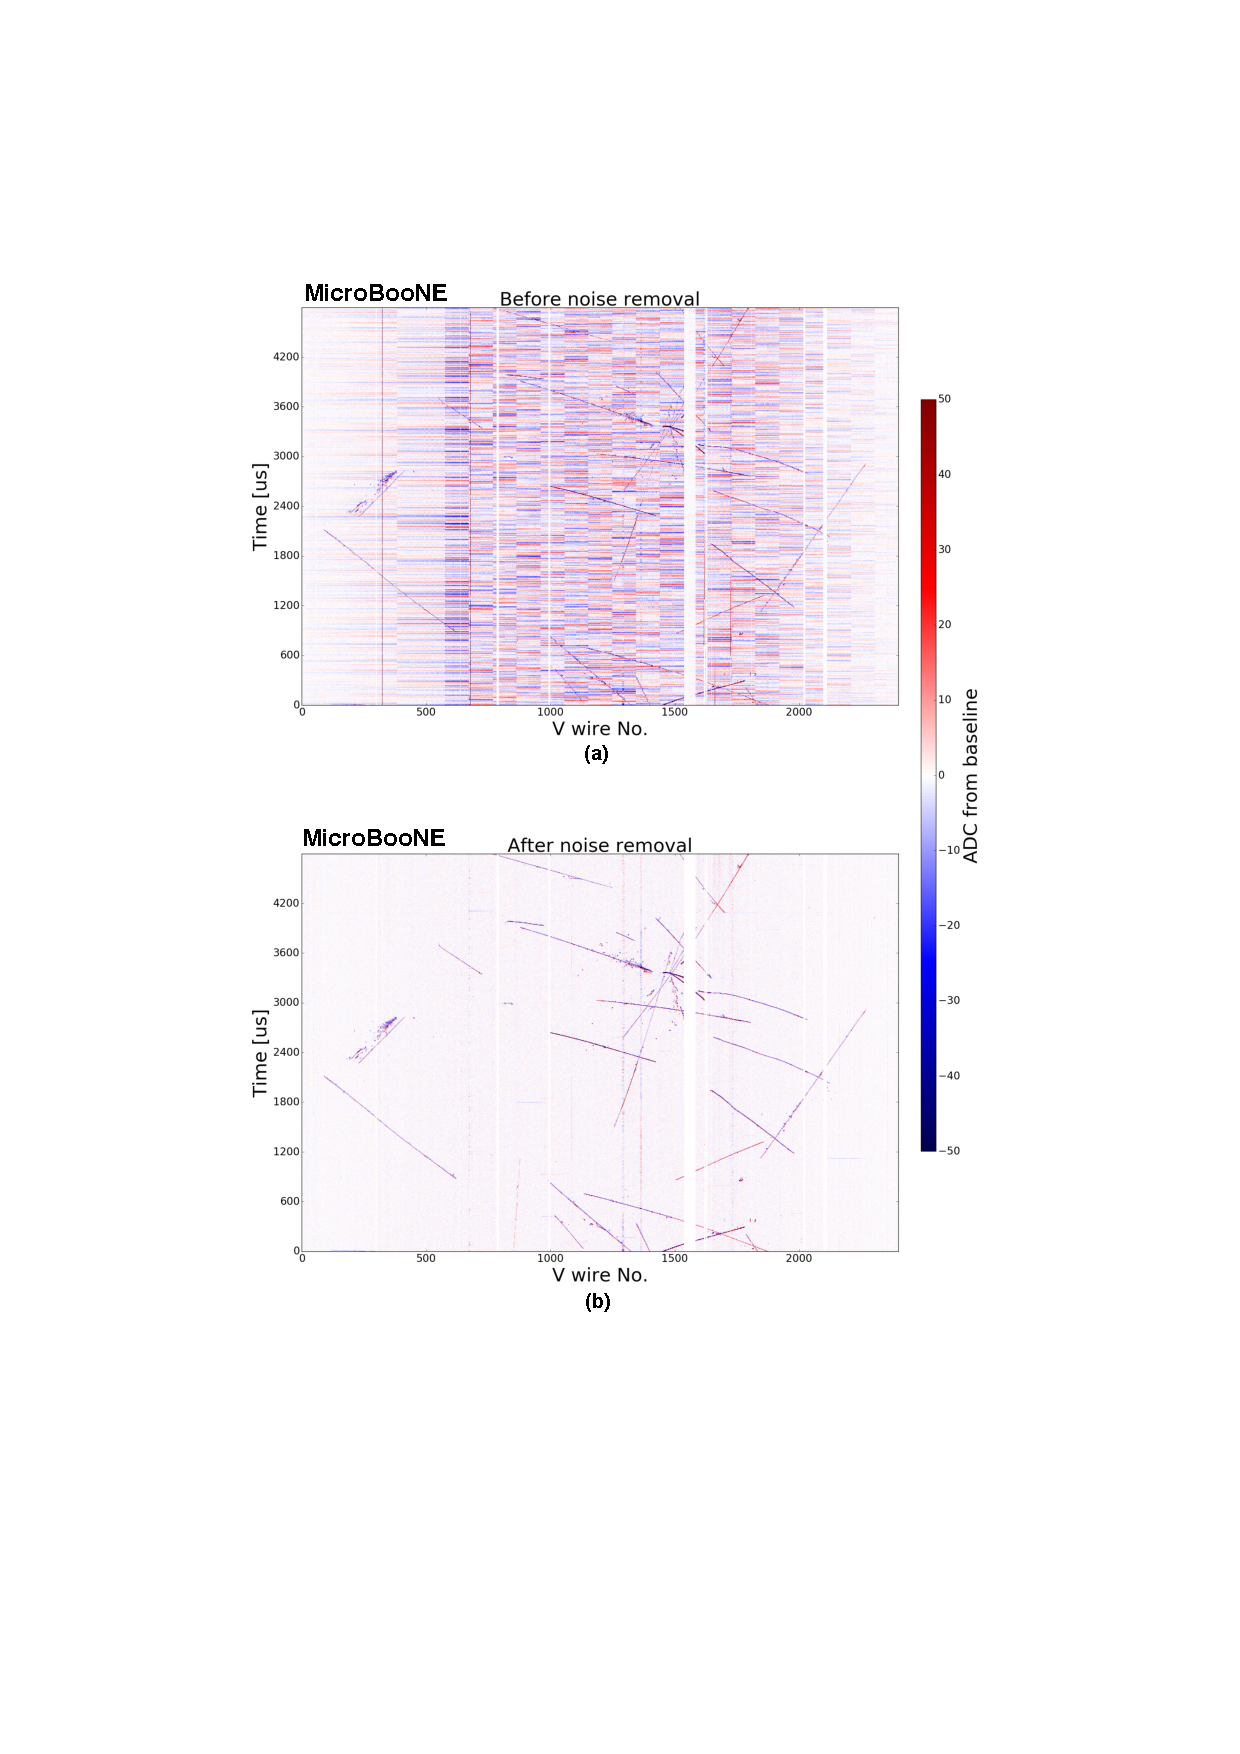
\includegraphics[width=0.75\linewidth]{figures/evd_noise.pdf}
    \caption{Data event display of the V induction plane showing the raw signal (a) before and (b) after offline noise filtering. From \cite{Acciarri:2017sde}.}
    \label{fig:evd_noise}
\end{figure}

\subsection{Signal deconvolution}
After the noise-filtering stage, a first reconstruction step aims to find regions-of-interest (ROI) in the wire signals. Thus, the signal deconvolution step aims to disentangle the detector electronic response from the original profile of the charge collected or induced on the wires. This process is usually performed by performing a Fourier transform of the measured signal, which yields:
\begin{equation}
    S(\omega) = \frac{M(\omega)}{R(\omega)},
\end{equation}
where $S(\omega)$ is the original signal, $M(\omega)$ is the measured signal, and $R(\omega)$ is the response function, all in the frequency domain. However, the response function typically decreases at high frequencies, leading to increased noise in this region of the frequency domain. This issue is solved by applying a filter function $F(\omega)$, whose details are thoroughly described in \cite{Adams:2018dra}. 

\subsection{Hit reconstruction}
The final stage of the signal processing tries to perform one or more Gaussian fits to the deconvolved signals. Each Gaussian fit corresponds to a \emph{reconstructed hit}. The time of the reconstructed hit is the mean of the Gaussian and its RMS corresponds to the Gaussian width. The integral of the fitted function gives the charge associated to the hit. Figure \ref{fig:evd_wires} shows a data event display of the collection plane, with the Gaussian fit to a waveform in the ROI. 
These reconstructed hits are finally passed to the pattern recognition framework, which aims to reconstruct 2D and 3D clusters. 

\begin{figure}[htbp]
    \centering
    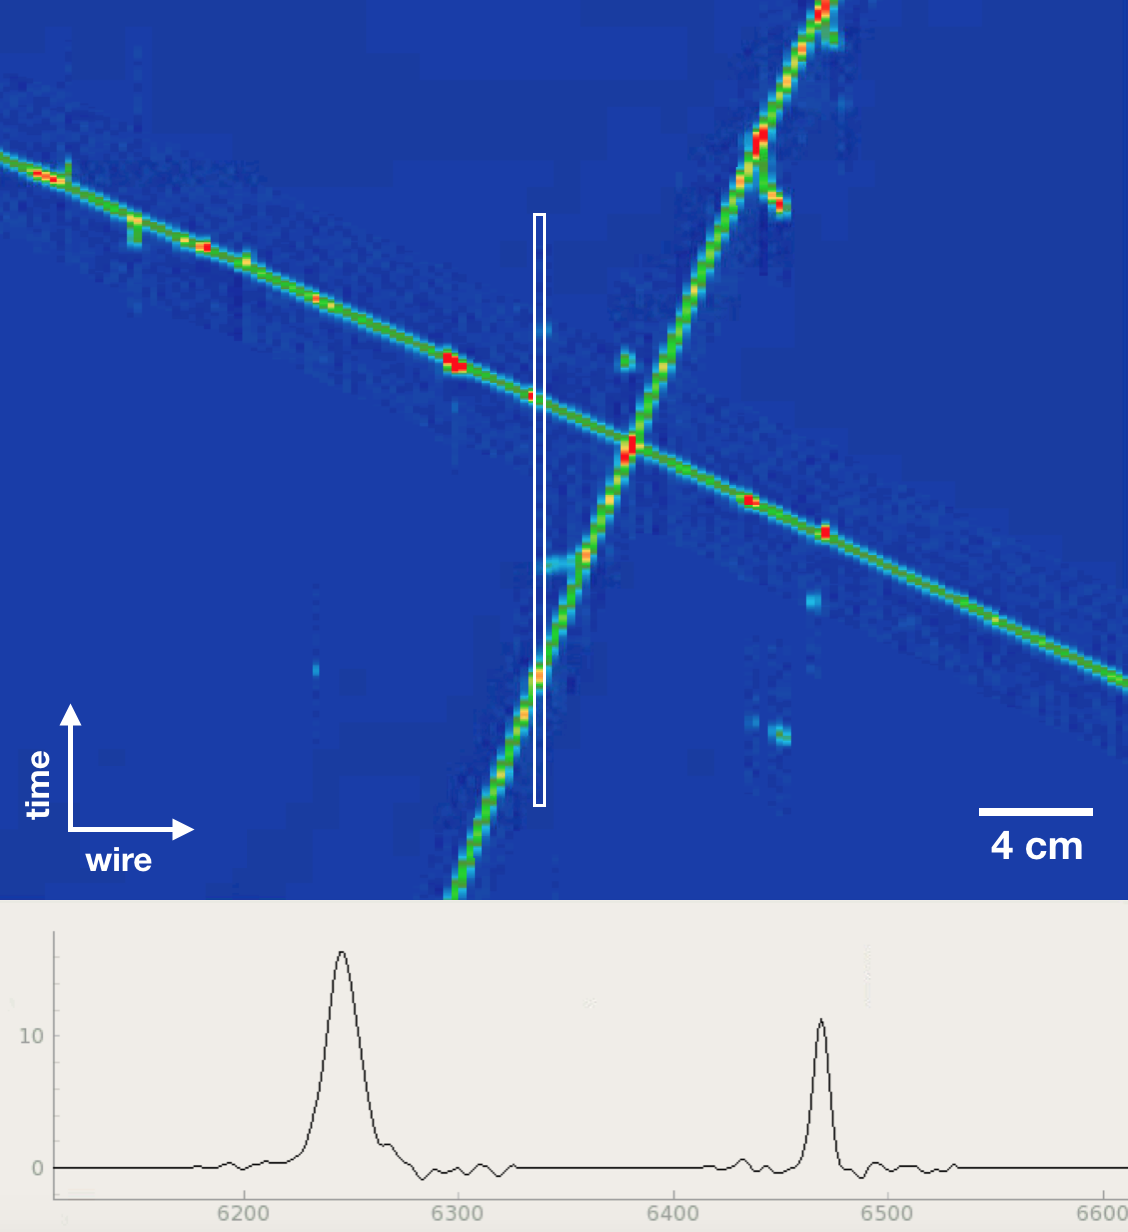
\includegraphics[width=0.75\linewidth]{figures/evd_wires.png}
    \caption{Data event display with a Gaussian fit to a waveform in a wire of the collection plane. The white box corresponds to the waveform in the bottom part. The units of the x-axis are in 500 ns time-ticks.}
    \label{fig:evd_wires}
\end{figure}

\section{The Pandora multi-algorithm pattern recognition}
The results shown in this document were produced using the Pandora Software Development Kit for pattern recognition. This general-purpose framework was specifically developed to identify energy deposits in high-granularity detectors, such as LArTPCs \cite{Marshall:2015rfa}.

Several algorithms are applied in sequence to the input information (in our case the reconstructed hits), which gradually build up a complete picture of the event.

As a first step, input hits are separated into three different lists, one for each plane. Then, for each list, an algorithm group together continuous and unambiguous lines of hits. These two-dimensional clusters are then examined by a series of topological algorithms. Given the presence of missing or unresponsive wires in the MicroBooNE detector, a continuous ionisation trail can be reconstructed as two or more separate clusters. The topological algorithms try to stitch different clusters together, if e.g. they point towards the same direction or if they are in close proximity. 

\begin{figure}[htbp]
    \centering
    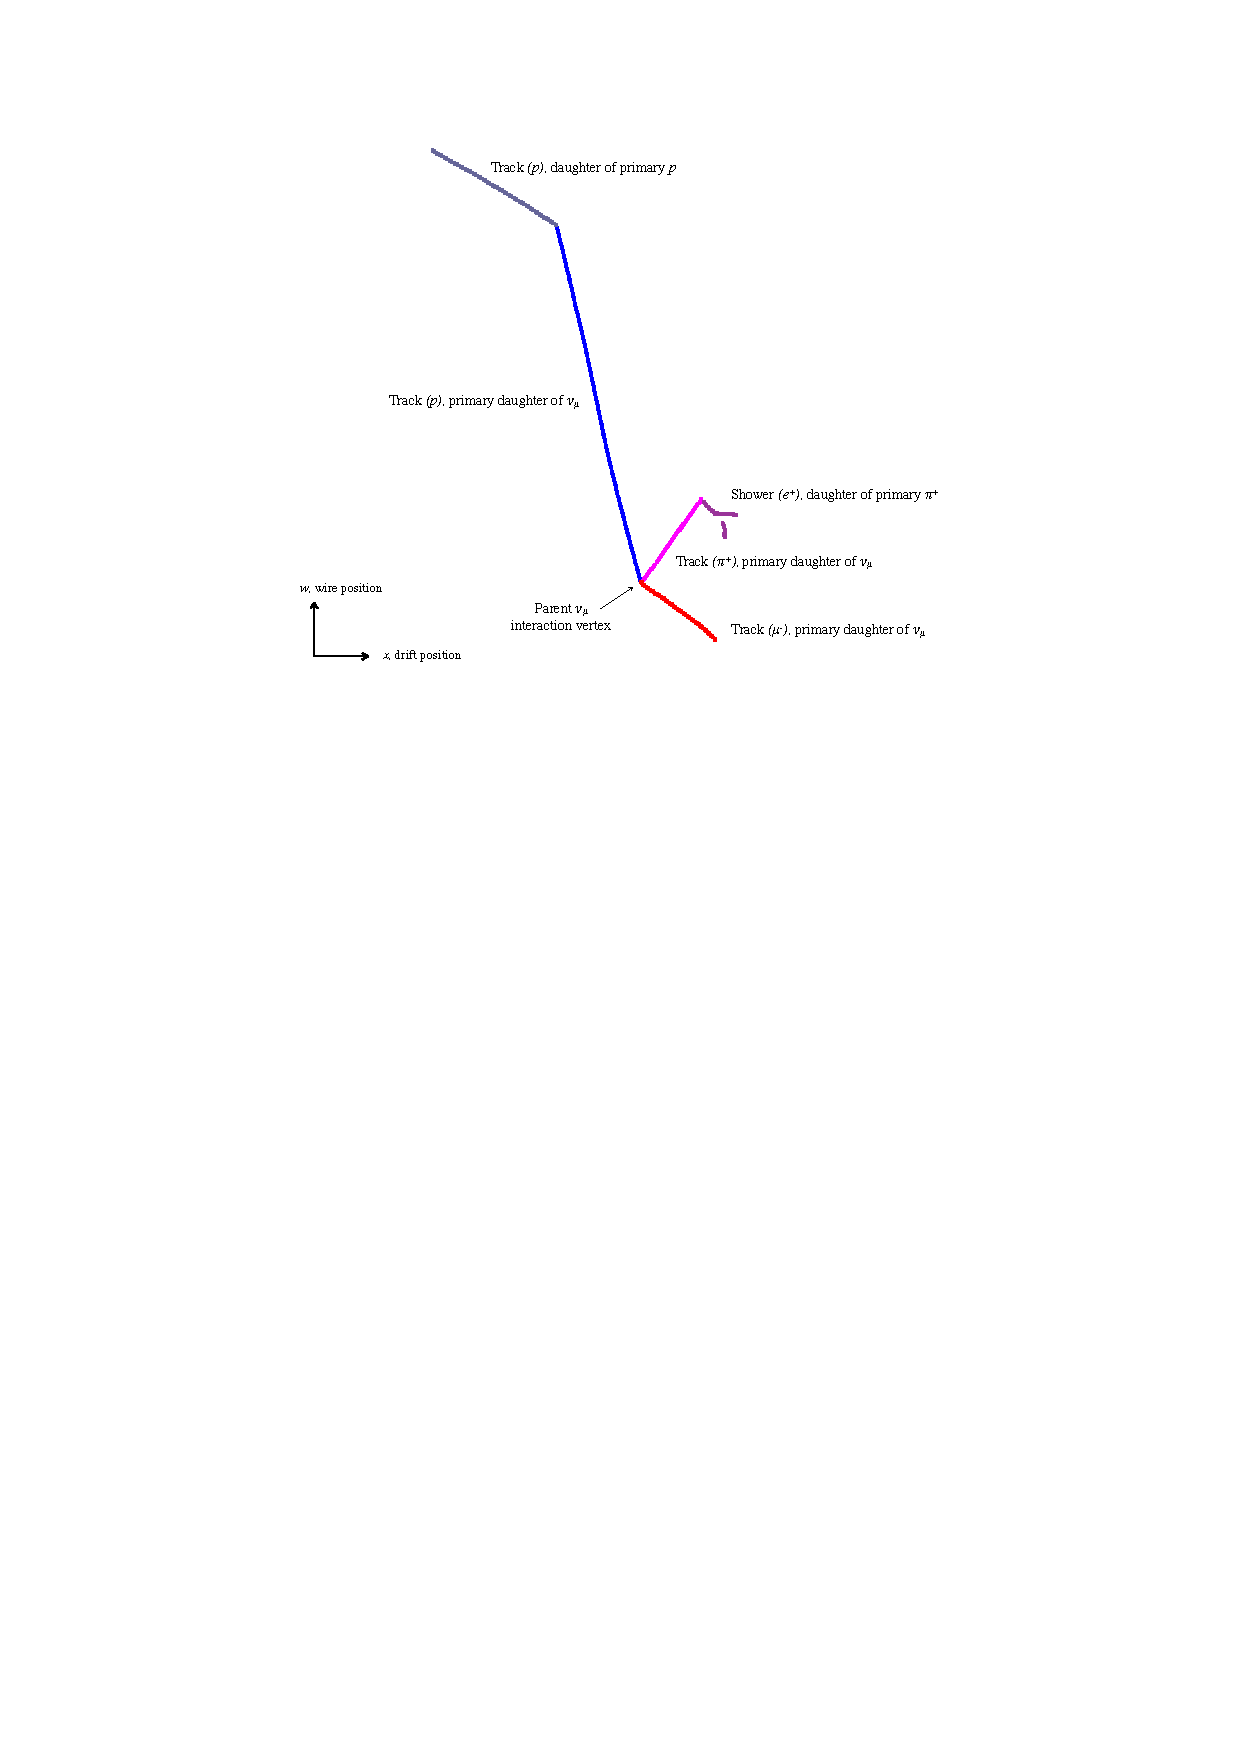
\includegraphics[width=0.75\linewidth]{figures/pandora_evd.pdf}
    \caption{Pandora pattern recognition output of a simulated CC $\nu_{\mu}$ event with a muon, a proton and a charged pion in the final state. Each particle is reconstructed as a separate cluster and the positron coming from the $\pi^+\rightarrow\mu^+\rightarrow e^+$ decay chain is classified as a daughter of the pion. From \cite{Acciarri:2017hat}.}\label{fig:evd_pandora}
\end{figure}

Once the topological algorithms deem the clustering in each plane as complete, the 3D reconstruction algorithms take as input the clusters from the three planes and aim to reconstruct the three-dimensional objects, which in Pandora are called \emph{PFParticles}.
Subsequently, a Support Vector Machine trained on Monte Carlo uses the topological and geometrical properties of the object to classify it as \emph{track} or as a {shower}. 
An important feature of the Pandora pattern recognition is its ability to create a hierarchy of reconstructed PFParticles. As an example, the reconstructed shower corresponding to a Michel electron will be considered as the daughter of the reconstructed track corresponding to the stopping muon. This capability is particularly important for the reconstruction of complex neutrino interactions, as exemplified in Figure \ref{fig:evd_pandora}.

Pandora can also run in two modes: one optimised for the reconstruction of cosmic rays and one optimised for the reconstruction of neutrino interactions. These two modes are used sequentially in our analysis in order to suppress the cosmogenic background, as described in Section \ref{sec:cosmicremoval}.